\chapter{Implementation and Performance of GAIA}
\newthought{The standard algorithms} for $b$ and $c$-jet tagging in the High Energy Physics community are MV1 and JetFitterCombNN respectively -- two neural networks batch trained using a variety of \emph{upstream} information about the particle collisions. Using the same features -- some basic likelihoods, vertexing information, and other signatures -- we show a significant improvement over MV1 and JetFitterCombNN. In addition, we show (albeit qualitatively) that the pretrained features extracted via the Stacked Denoising Autoencoder cluster and show separation between bottom and light jets. First, we provide a brief description of the implementation of GAIA, then we discuss benchmarking and performance measures on the classification task.

\section{Design and Implementation of GAIA}
GAIA was implemented with speed, portability, modularity, and expandability in mind. In addition to development on the algorithms side -- i.e., Deep Learning, we integrate GAIA into the ROOT \citep{ROOT} Framework for High Energy Physics Data Analysis. Simulations and data within CERN are stored in a ROOT structure called a \texttt{TTree}. We provide a simple wrapper around the native CERN I/O system to make training, testing, and validation easier, and more in line with the mathematical formulation.

The GAIA framework was written in C++ using two standards for two separate parts. The main interface was written using C++11 standard. Specifically, the \texttt{<utility>} and \texttt{<memory>} headers were used for R-Value references and smart pointer (\texttt{std::unique\_{}ptr}) functionality, the \texttt{<random>} header was used for random number generation, and range-based for-loops were used, as the compiler used (GCC 4.8.X) optimized all iterations using this structure when the \texttt{-O3} flag is passed. The header-only thin-client library uses the C++0x standard to ensure compatibility with the existing CERN software.

All trainings and testings of the GAIA framework were run on the Omega Supercomputing Cluster\footnote{Omega Cluster Platform 3000 BL460c G6, Xeon X5560 4C 2.80GHz, Infiniband QDR} at Yale University. A typical training time for a 7 layer Deep Network with full training on stacked, denoising autoencoders over 30 million samples was around 2 hours. 

We provide a \texttt{Layer} class which encapsulated all operations relating to equations \eqref{net_prediction} and \eqref{auto_soln}, allowing for functionality with or without feature learning. Specifically, the \texttt{Layer} class holds $W_i$ and $\mathbf{b}_i$ The \texttt{Layer} class also is responsible for all parameter manipulation, and offers methods for setting parameters such as learning rate, etc. For a presented input $\mathbf{x}$, the \texttt{Layer} class offers a method called \texttt{Layer.feed(std::vector<double> x)} which forms and stores $\mathbf{z^{(i)}} = W_i \mathbf{x}+{b}_i$ and $\mathbf{a}^{(i)}=f(\mathbf{z^{(i)}})$. Also noteworthy is the fact that the activation function $f$ is passed as a function pointer to the method within the constructor, making user-preference for a specific type of activation function more feasible.

We also provide an \texttt{Architecture} class, which provides a generic method of combining arbitrarily sized \texttt{Layer} objects into a network structure. It also handles all data passing between layers, and mediates the greedy feature learning within the neural network. Its main purpose is to provide the backpropagation function to the neural network. Build on top of the \texttt{Architecture} class is a \texttt{NeuralNet} class, which provides API sugar around many of the methods and provided functionality. The \texttt{NeuralNet} class also provides a mediatory layer between the user and the \texttt{Dataset} class, which serves as the wrapper around the native CERN \texttt{TTree} data structure. Thus, a user will only need to interact with the \texttt{NeuralNet} class from data loading to training to testing. We now walk through a simple example to illustrate the functionality of the API. Suppose we have a ROOT file named \texttt{dataset.root} containing a \texttt{TTree} called \texttt{MyTree}. Suppose we want to predict the outcome called \texttt{"output"} from the variables called \texttt{"var\_1"}, \texttt{"var\_2"}, and \texttt{"var\_3"}, and all of these variables are within the \texttt{TTree} called \texttt{MyTree}. Now suppose we want to build a neural network with one hidden layer, say with two nodes. The following code will do this. 

\begin{small}
\begin{verbatim}
#include "NeuralNet.h"
#include <TFile.h>
#include <TTree.h>

int main(int argc, char const *argv[])
{
    // Make a neural net with 3 inputs, 2 hidden nodes
    // and one output
    std::vector<int> structure = {3, 2, 1};

    // Initialize the network
    NeuralNet Net(structure);

    // The first argument is the root file and
    // the second argument is the name of 
    // the TTree
    Net.set_dataset("dataset.root", "MyTree");

    // The first argument is the variable name
    // and the second argument is its numeric type
    Net.set_input_branch("var_1", "double");
    Net.set_input_branch("var_2", "double");
    Net.set_input_branch("var_3", "double");

    // Same for outputs.
    Net.set_output_branch("output", "double");

    // Find the transform so that inputs are of
    // zero mean and unit variance.
    Net.getTransform();

    // Train for 5 epochs, using 1000 points
    // and save the configuration to a file
    // called "neuralnetwork.nnet"
    Net.train(5, 1000, "neuralnetwork.nnet");

    return 0;
}

\end{verbatim}
\end{small}



As we can see, the interface is straight-forward, and additional functionality is elaborated upon in documentation. 

\section{Measuring Performance}


To benchmark the performance of GAIA with respect to the current selection of other particle classifiers,  we use some standard measures of classifier performance. We make these metrics very problem dependent for the sake of concreteness. We denote the quarks / jets that we try to identify as $\{b,c,u\}$ for Bottom, Charm, and Light jets respectively. These will be henceforth referred to as "flavors". For a given threshold -- called a "cut" within High Energy Physics -- on any number of output discriminants, define the efficiency of such a cut with respect to a certain flavor to be the number of jets of such a flavor that pass the discriminant out of the total number considered. We say that a jet or quark \emph{passes a cut} if its value of the discriminant is higher than the threshold or cut value.  Denote this efficiency quantity as $\epsilon_\theta$, for $\theta\in\{b,c,u\}$. This can be more succinctly formulated as
\begin{equation}
\epsilon_\theta = \frac{\text{\# of }\theta\text{ jets passing the cut in sample}}{\text{Total \# of }\theta\text{ jets in sample}}
\end{equation}
 with respect to some cut on some combination of discriminants. To measure purity, we also consider the \emph{rejection} of a cut with respect to some flavor $\theta$, $r_\theta$, which is simply defined as the reciprocal of the efficiency. That is $r_\theta = 1 / \epsilon_\theta$.
 
For a particular type of identification problem -- that is, for $c$-tagging or $b$-tagging, we always consider the efficiency of the signal and the rejection of the two backgrounds. For any level of signal efficiency, it is always desirable to maximize the background rejection for both types of background. 

For a physics analysis, we cannot simply take the Maximum A Posteriori (MAP) estimate of class membership, as different analysis groups need different levels of purity or yield, and some groups have a very different sample composition. For example, a group needing to identify $b$-jets against a background that is primarily $u$-jets is going to need a very different discriminant than an analysis group needing to separate $b$-jets from an even mix of $c$ and $u$-jets. 

Consider our particular classifier, with outputs $p_u, p_b$, and $p_c$ representing the posterior probabilities that an observation is a light jet, bottom jet, or charm jet respectively. The posterior space has a distribution $f_{p_u,p_b,p_c}(p_u, p_b, p_c)$ over all outputs, and individual distributions for each $\theta$, $f_\theta(p_\theta)$. Suppose our signal is $\theta$. We then can construct a set of discriminants
\begin{equation}
D = \{ \log(p_\theta / p_\nu) : \nu \in \{u,b,c\}, \nu \neq \theta \}.
\end{equation} 
In our particular case, this leaves two discriminants for a three class problem. Note that we take a $\log(\cdot)$ here simply to make any even sampled cuts on this distribution more evenly sampled. 

In the case of $b$-tagging, we refer to $\log(p_b/p_c)$ as the anti-$c$ discriminant, and we refer to $\log(p_b/p_u)$ as the anti-$u$ discriminant. In the case of $c$-tagging, we refer to $\log(p_c/p_b)$ as the anti-$bottom$ discriminant, and we refer to $\log(p_c/p_u)$ as the anti-$u$ discriminant. Note that for every pair of discriminants, we obtain a signal efficiency and two background rejections. We can use a \emph{Receiver Operating Characteristic} (ROC) curve to examine the relationship between efficiency and rejection. To form the ROC curve we essentially form a 2D histogram of the output logarithmic discriminants, and can use cumulative counts to determine efficiency and rejection for each flavor. 

In the $c$-tagging case, we use a special plot called an iso-efficiency contour\footnote{Credit for the idea for this plot goes to Daniel H. Guest}, which shows the $c$-tagging efficiency as a surface over a plane of light rejection and bottom rejection. Such curves can be divided to show the ratio of efficiencies between $c$-taggers.

\subsection{Sensitivity to $p_T$ and $\eta$}

The usage of a classifier is relatively unique within physics. Since any classifier will have to probe and classify on datasets that are of different $p_T$ and $\eta$ ranges, care must be taken to ensure that a classifier isn't overfitting to a particular $(p_T,\eta)$ combination. Consider the following. Suppose we let a classifier learn the fact that low $p_T$ jets tend to be light jets and higher $p_T$ jets tend to be $b$-jets. Then, the model will call everything below a certain $p_T$ a light jet, maximizing overall accuracy. However we want our performance to be as even as possible across the $p_T$ and $\eta$ spectrum, as will be elaborated upon in Section \ref{sec:btag}, as the classifier must be able to perform well in different areas of the support.

\subsection{Choosing What to Learn, Revisited}

Using \emph{online physics reweighting}, we can dictate what features our pretraining discovers. We can also dictate to what degree our \nn{} should balance out biases in distributions over the kinematic variables $p_T$ and $\eta$. Using the reweighting outlined in Chapter 3, we reweight such that the distributions $f(p_T, \eta, c)=f(p_T, \eta, b)=f(p_T, \eta, u)$. We then show two things -- first, that the features learned by the stacked, denoising autoencoders show clustering based on flavor type, and second, that the reweighting scheme ensures that performance stays at reasonable levels across the $p_T$ spectrum. The latter of these two will be elaborated upon in Section \ref{sec:btag}.

How can we visualize the features we learn through the unsupervised, unlabelled process? We look at samples unseen during the unsupervised learning procedure, and map them to the new feature space using the structure in the network. 

\begin{FPfigure}
\includegraphics[width=\textwidth]{figures/gaia.features}\\
\includegraphics[width=\textwidth]{figures/gaia.features.IDNE}
\caption[The ATLAS detector]{Feature space of the original dataset Learned by GAIA without (top) and with (bottom) Inverted Deep Network Encoding. Bottom Jets are red, Light Jets are blue, and Charm Jets are green.
\label{fig:featGAIA}}
\end{FPfigure}


Consider Figure \ref{fig:featGAIA}, which shows the separation of flavor types in the case where we use IDNE (bottom) and where we do not (top). In both cases, we can clearly see that there is separation between light jets and bottom jets, albeit the features learned by GAIA with IDNE show an almost-linearly-separable class discriminator. However, we can see that the features learned by GAIA with IDNE show a separation for charm jets, which shows a greater ability to learn and denoise latent features present within the data. The idea of feature learning assumes that for every observed  $\mathbf{x}\in\R^D$, there is a vector $\mathbf{y}\in\R^d$, with $d<D$, along with a mapping $\varphi:\R^D\longrightarrow\R^d$ such that $f(\mathbf{y}) \approx \mathbf{x}$. In our case, we assume that a 3D feature space can generate all observed features we see within the detector. We see that in the case of IDNE, the features learned seem to be more aligned with type, which leads to the conclusion that the features are more explanatory, though this itself warrants a study.

\subsection{A Learning Process}

We now move away from feature learning and consider the discriminatory power and potential for GAIA within a physics analysis group. To measure the performance and potential of GAIA within a physics context, we compare the performance of GAIA on the two key identification tasks -- $c$-tagging and $b$-tagging -- to the current standards within the ATLAS, MV1 for $b$-tagging, JetFitterCharm for $c$-tagging, and JetFitterCombNN for general purpose tagging.

The variables used to JetFitterCombNN are $p_T$, $\eta$, and the so-called JetFitter variables, a reconstruction algorithm that parses particle tracks out of energy deposits. JetFitterCombNN produces $p_b$, $p_u$, and $p_c$ posteriors from these inputs. The MV1 tagger uses the $p_b$, $p_u$, and $p_c$ outputs from JetFitterCombNN, and uses the IP3D and SV1 likelihoods as inputs, and produces one output -- $p_b$. JetFitterCharm uses the JetFitter variables with a tuning to better identify charm jets, and produces $p_b$, $p_u$, and $p_c$ posteriors. We train GAIA to use the IP3D and SV1 likelihoods, $p_T$ and $\eta$, the normal JetFitter variables, and the charm-tuned JetFitter variables while ignoring the posteriors from JetFitterCombNN that MV1 uses. The reason to avoid using the posteriors from JetFitterCombNN is simple -- we use it's input, and thus, we should be able to learn the relationship learned by JetFitterCombNN. In addition, each tagger must be calibrated, and interdependencies slows down production.  

We now elaborate upon some semantics and details of the training benchmarking process. The tagger presented in this thesis is often referred to as simply GAIA, even though this is the name of the software framework. The structure of the GAIA tagger is as follows. We use 27 input variables, we have feature layers of size 30, 19, 11, and 5, and we map to 3 posteriors. We first map to a feature layer of 30 features to allow for redundancies in the learning of the input distribution. 

We utilize a Monte Carlo sample for training and testing -- specifically, we use the \texttt{PowhegPythia} generator, and the \texttt{mc12\_8TeV.117050.PowhegPythia\_P2011C\_ttbar.skim\_p1562\_v0.130731164806} dataset. We use 25 million training jets, and 5 million validation jets, randomly partitioned. The plots shown here are generated for one particular training of GAIA, and is representative of overall performance. We train for  100 epochs for the following reason. Since we add noise to features in pretraining and in supervised training, we do not overfit. We can train for more than 100 epochs, but experience says that epochs beyond 100 do not contribute to performance.

Some performance plots will show "GAIA B" and "GAIA C", which are simply different tunings of the reweighting. GAIA C is a more generic tagger and is weighted for $b$ and $c$ tagging -- that is, flavor dependent $p_T$ and $\eta$ distributions are forced to be the same. GAIA B is a tagger more specifically tuned for $b$-tagging, and for a search such as $H\longrightarrow bb$, which relies on being able to tag low $p_T$ $b$-jets. The weighting scheme in this instance doesn't force the distributions to be equal -- we let low $p_T$ light jets retain some imbalanced influence. Also note that GAIA with IDNE is not included in most plots, as it new has not been tested enough to be included in the next ATLAS data reprocessing. There will be a short section at the end that shows some preliminary, promising results using GAIA with IDNE, and we withold a complete exposition until further testing. 

To get a sense of class-based separation over the posterior probabilities learned by GAIA, consider Figures \ref{fig:bpost}, \ref{fig:upost}, and \ref{fig:cpost}, which show the log count histograms of the posterior probabilities of each flavor, with color overlay indicating true flavor membership of the jet. As is evident in Figure \ref{fig:bpost}, the value $p_b$ seems to hold a lot of discriminatory power, especially for high values of the discriminant. This means that for lower efficiencies, the rejection values we obtain should yield a pure passing sample. In Figure \ref{fig:upost}, we see the $u$ posterior probability colored by true flavor. This posterior also holds a significant amount of information. In addition, it seems as though the $p_u$ posterior seems to hold equal discriminatory power over $b$ and $c$ jets. In Figure \ref{fig:cpost}, we see the $c$ jet posteriors colored by true flavor. Here we can see first hand the difficulty associated with $c$-tagging. Though we clearly have some discriminatory power, it seems as though on its own, $p_c$ will not produce results of merit by itself, necessitating the use of the aforementioned log ratios of posterior probabilities. 



\begin{figure}[h]
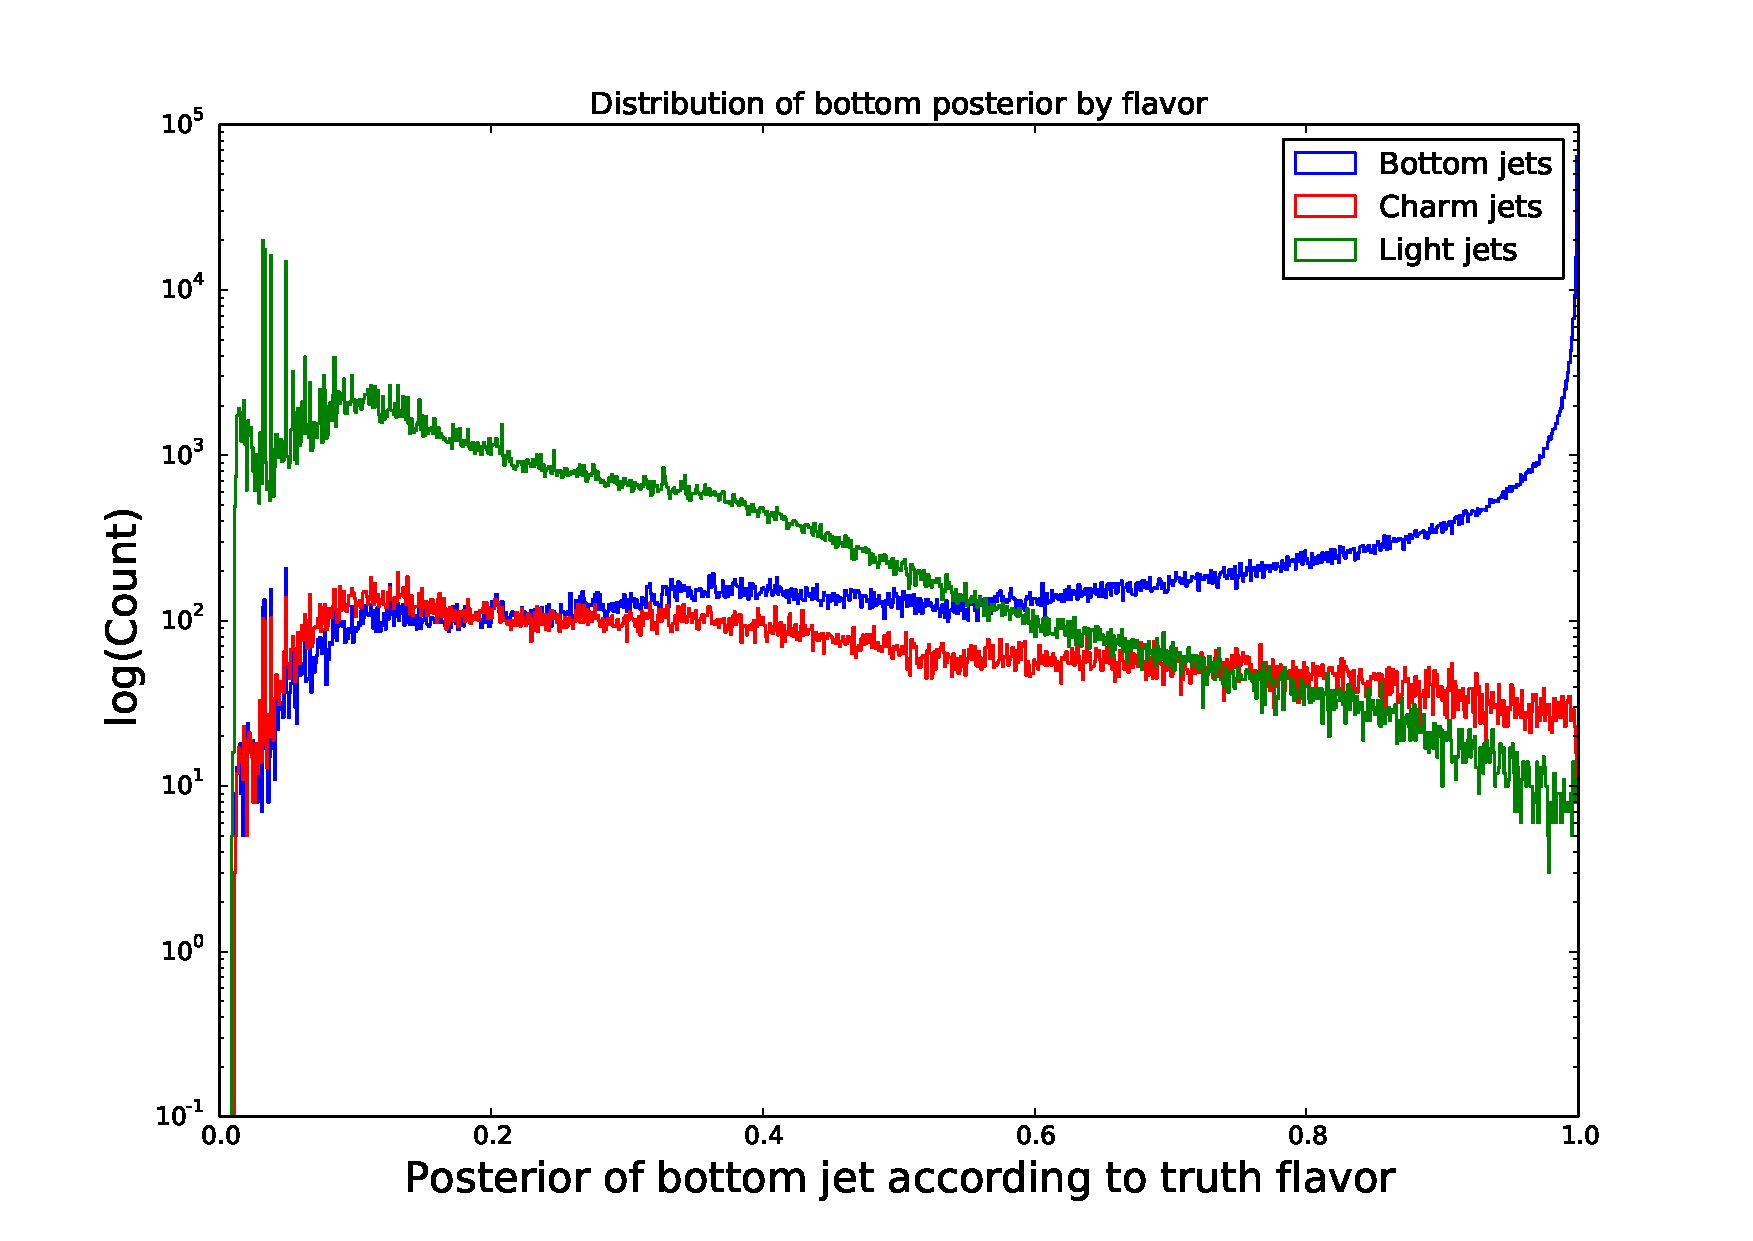
\includegraphics[width=\textwidth]{figures/unweight_bottom_p_distro}
\caption[The ATLAS detector]{$b$ posterior probability from GAIA by flavor.
\label{fig:bpost}}
\end{figure}

\begin{figure}[h]
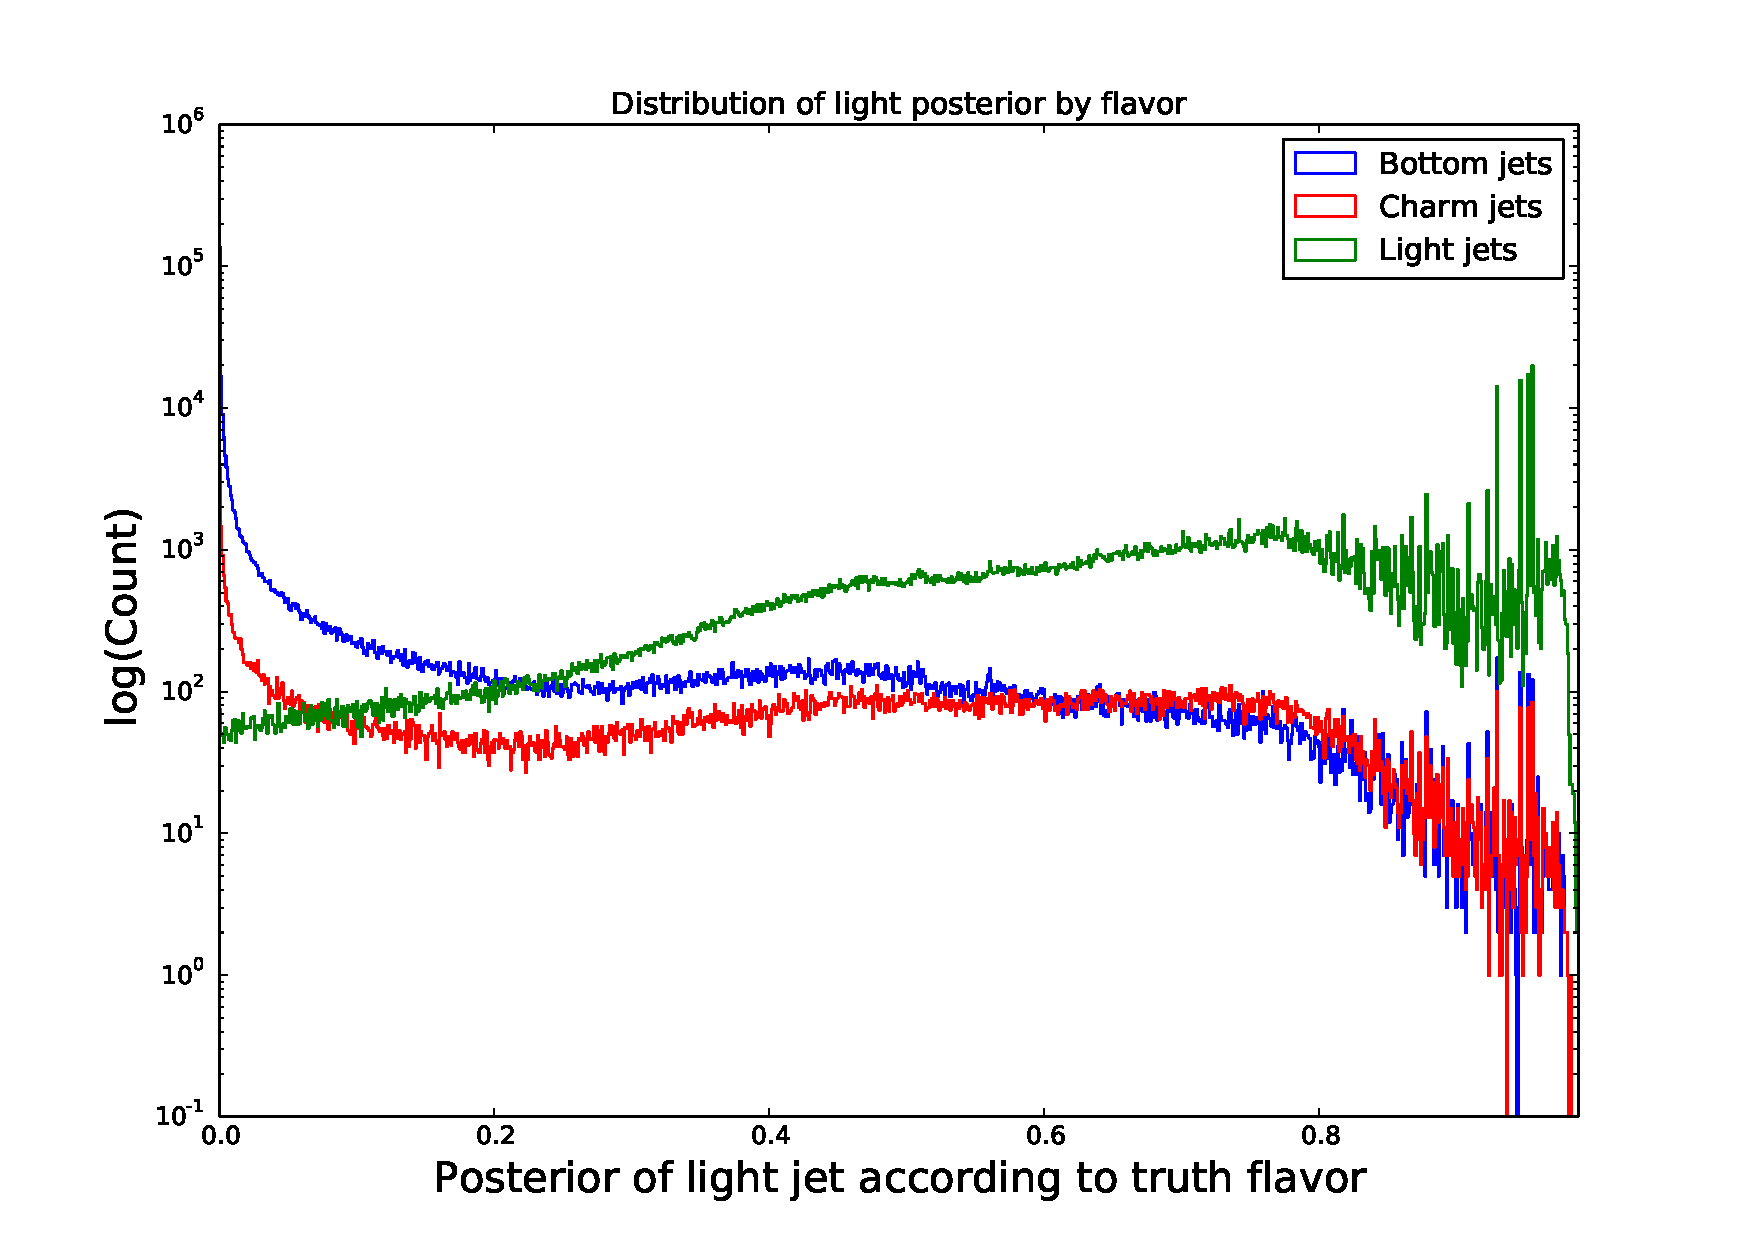
\includegraphics[width=\textwidth]{figures/light_p_distro}
\caption[The ATLAS detector]{$u$ posterior probability from GAIA by flavor.
\label{fig:upost}}
\end{figure}

\begin{figure}[h]
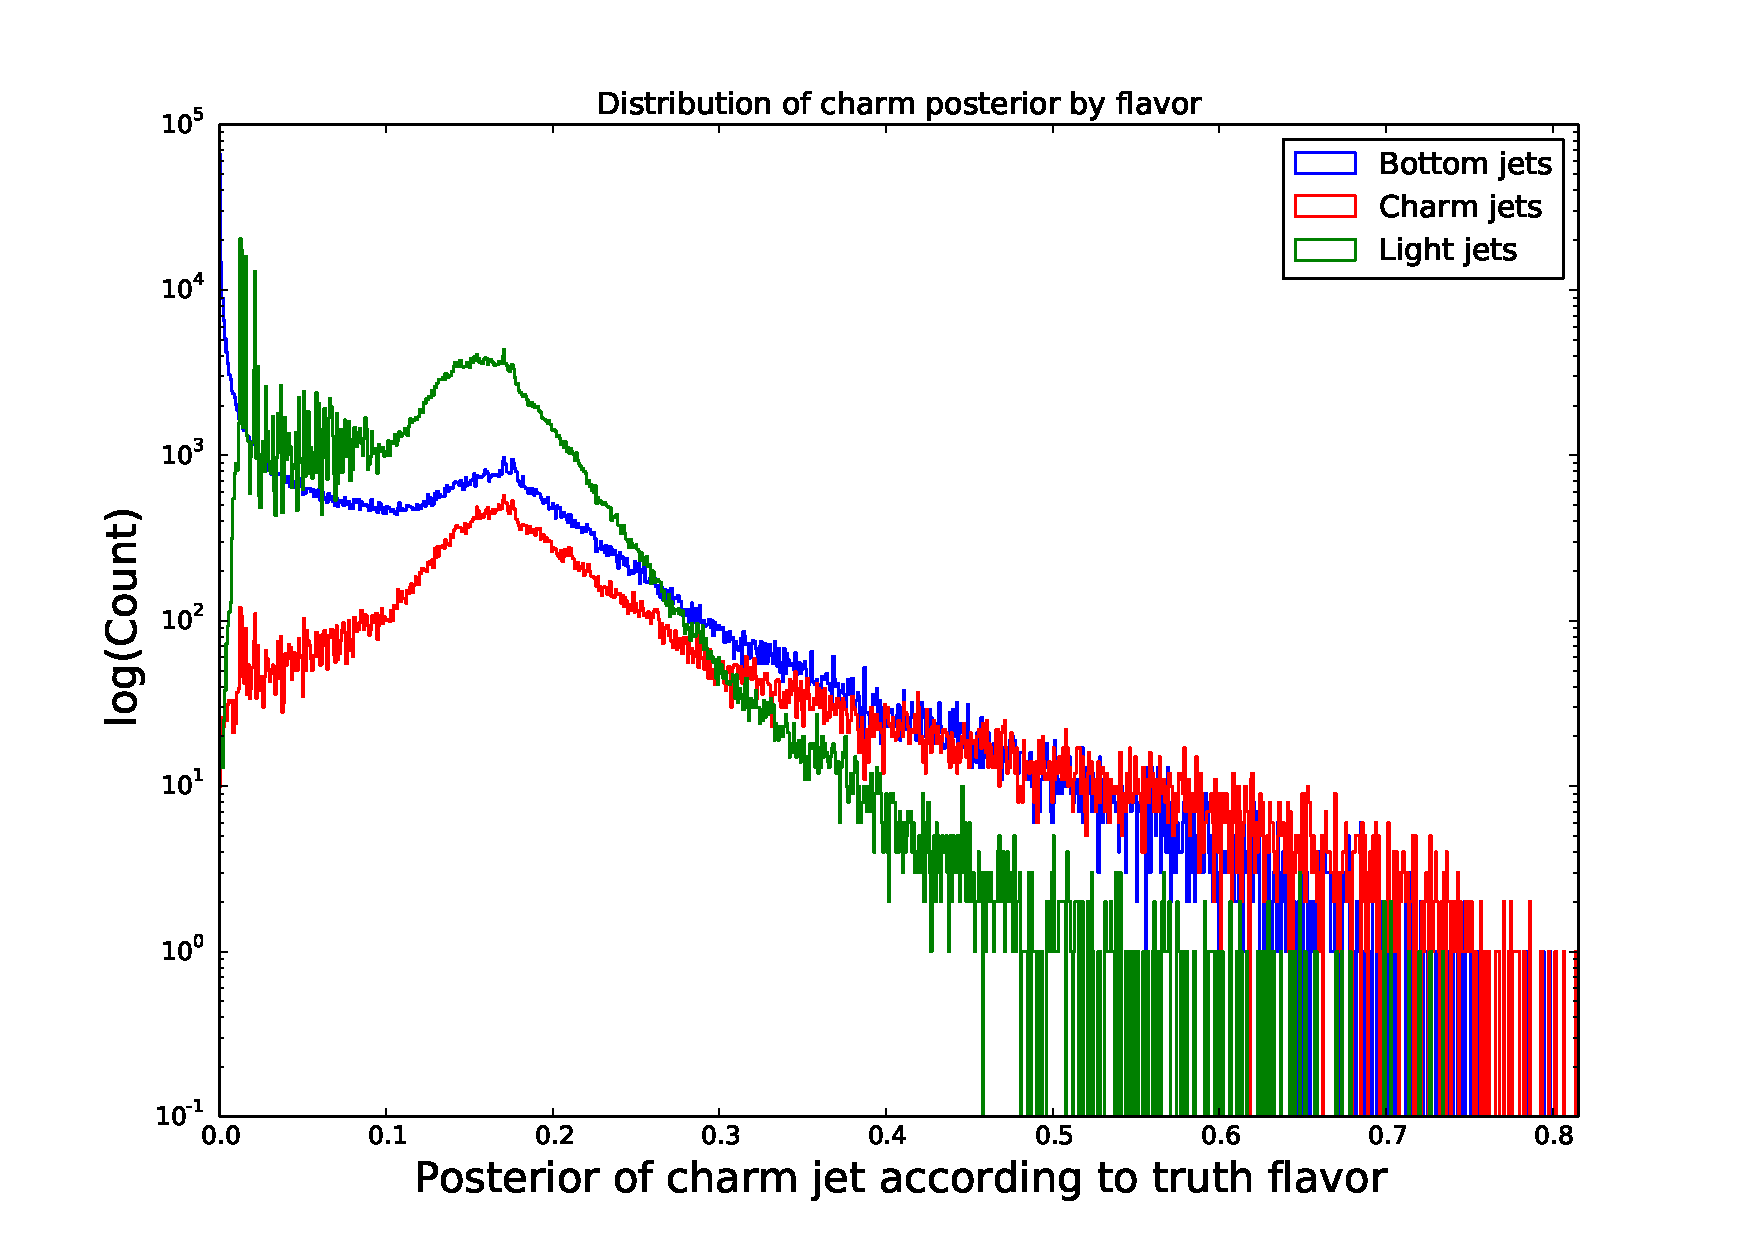
\includegraphics[width=\textwidth]{figures/charm_p_distro}
\caption[The ATLAS detector]{$c$ posterior probability from GAIA by flavor
\label{fig:cpost}}
\end{figure}



\section{$b$-tagging} 
\label{sec:btag}

\newcommand{\roc}{Receiver Operating Characteristic }
\newcommand{\er}{$\varepsilon$-r }

To determine the viability and potential performance improvements that GAIA offers over the current ATLAS line-up of taggers, we compare GAIA to all three benchmark taggers. In particular, we first construct \roc curves for each tagger. For MV1, there is a single discriminant, so our \roc will simply be a line running through \er space\footnote{Efficiency-Rejection}. However, for each of the other taggers, we have two discriminants on which we make cuts. Thus, we end up with a non-line subset of \er space. To make comparison easier, for each efficiency, we take the maximum of all possible rejection values, knowing that the other values of the rejection represent a tradeoff between the different types of background rejection.

\subsection{Whole Sample Performance}
\begin{figure}[h]
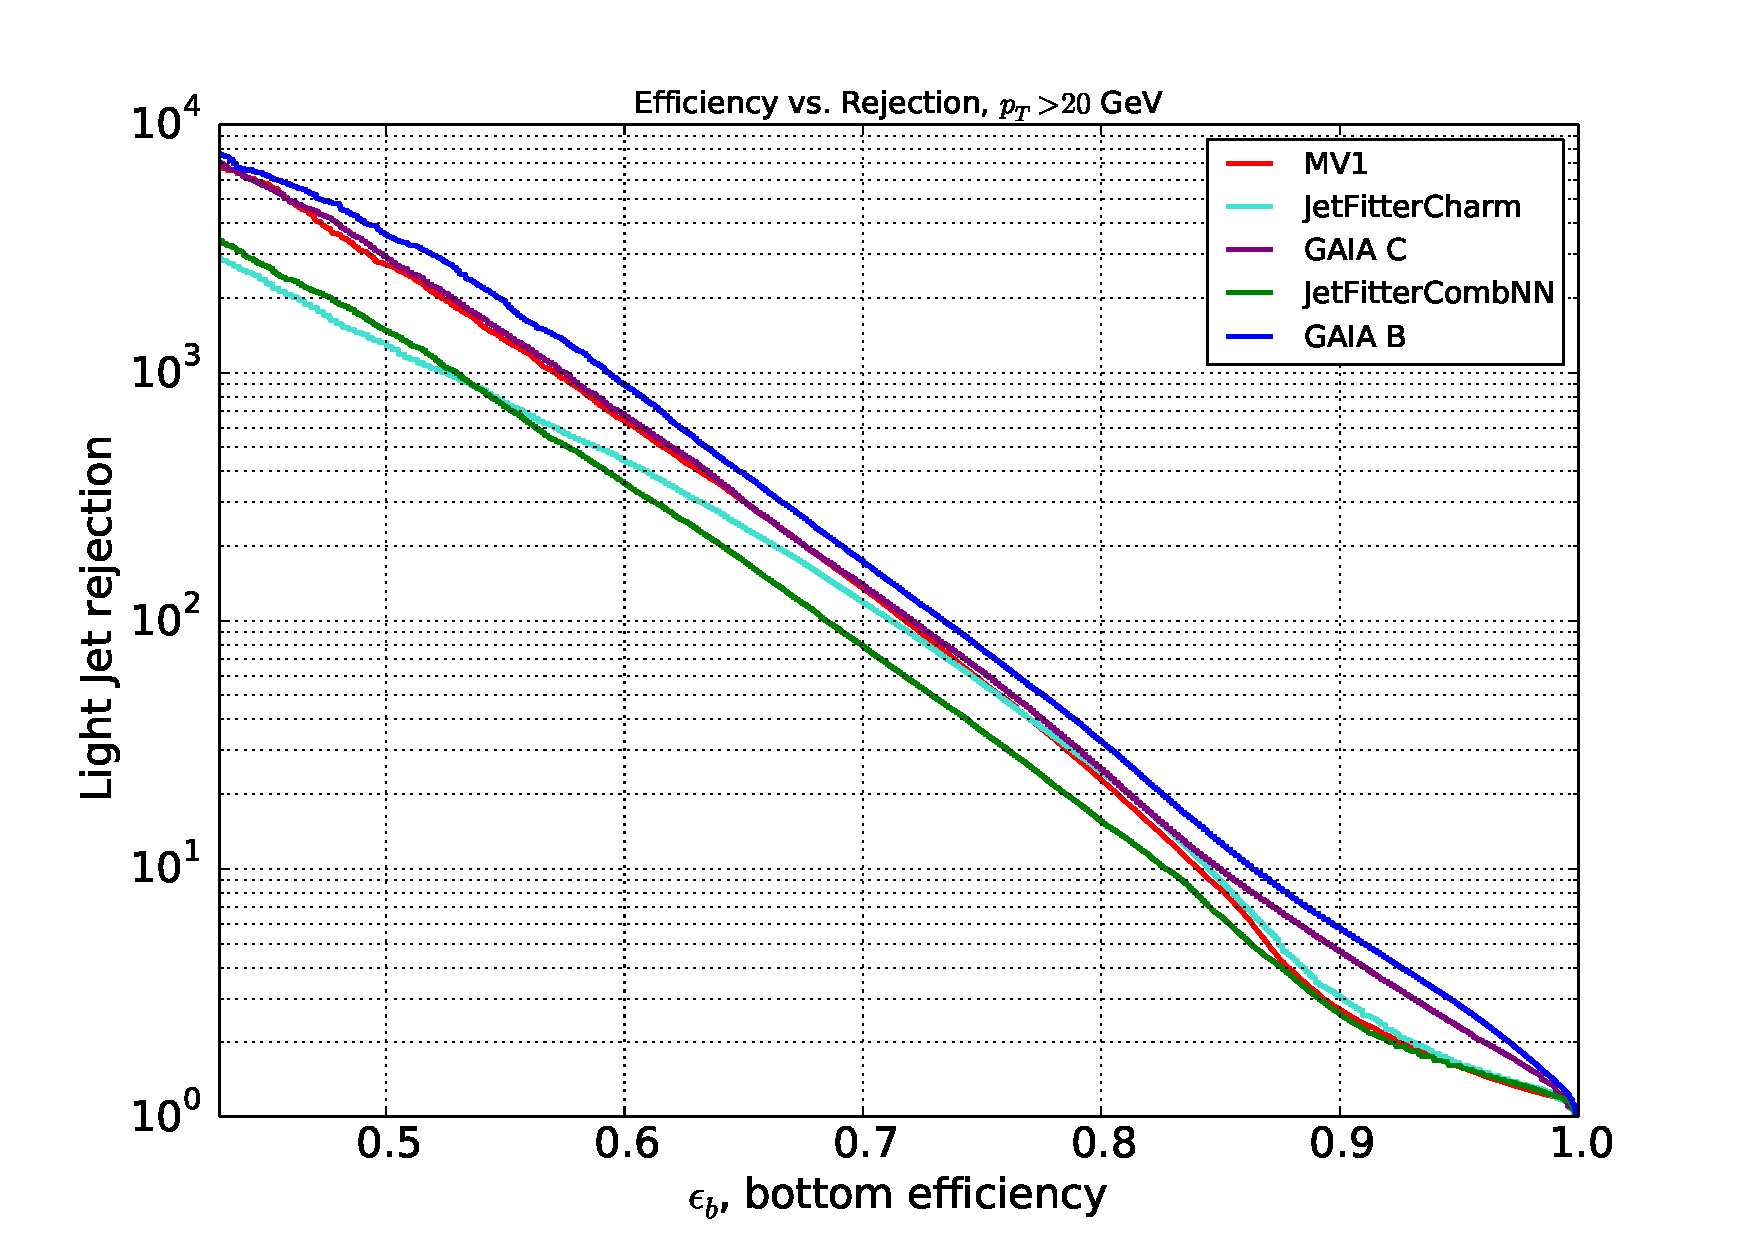
\includegraphics[width=\textwidth]{figures/btag/u_rej_ROC.pdf}
\caption[The ATLAS detector]{$u$-rejection Receiver Operating Characteristic Curve of Tagging Lineup.
\label{fig:urejROC}}
\end{figure}

Figure \ref{fig:urejROC} shows the light jet rejection \roc of each algorithm, and we see that both GAIA B and GAIA C have a higher rejection value for each efficiency of interest \footnote{We only care about $\varepsilon>0.5$ for physics related reasons.}, indicating that GAIA can offer better light rejection across all values of $\varepsilon$. Notice that this convex hull of possibilities for taggers that use three posteriors represents a cut only on $\log(p_b/p_u)$.

Next, consider the rejection of the other background for $b$-jet identification -- charm jets. Figure \ref{fig:crejROC} shows the convex hull of possibilities in \er space for charm rejection, Notice that in this instance, the only discriminant used for JetFitterCharm, JetFitterCombNN, and GAIA B and C is $\log(p_b/p_c)$.

\begin{figure}[h]
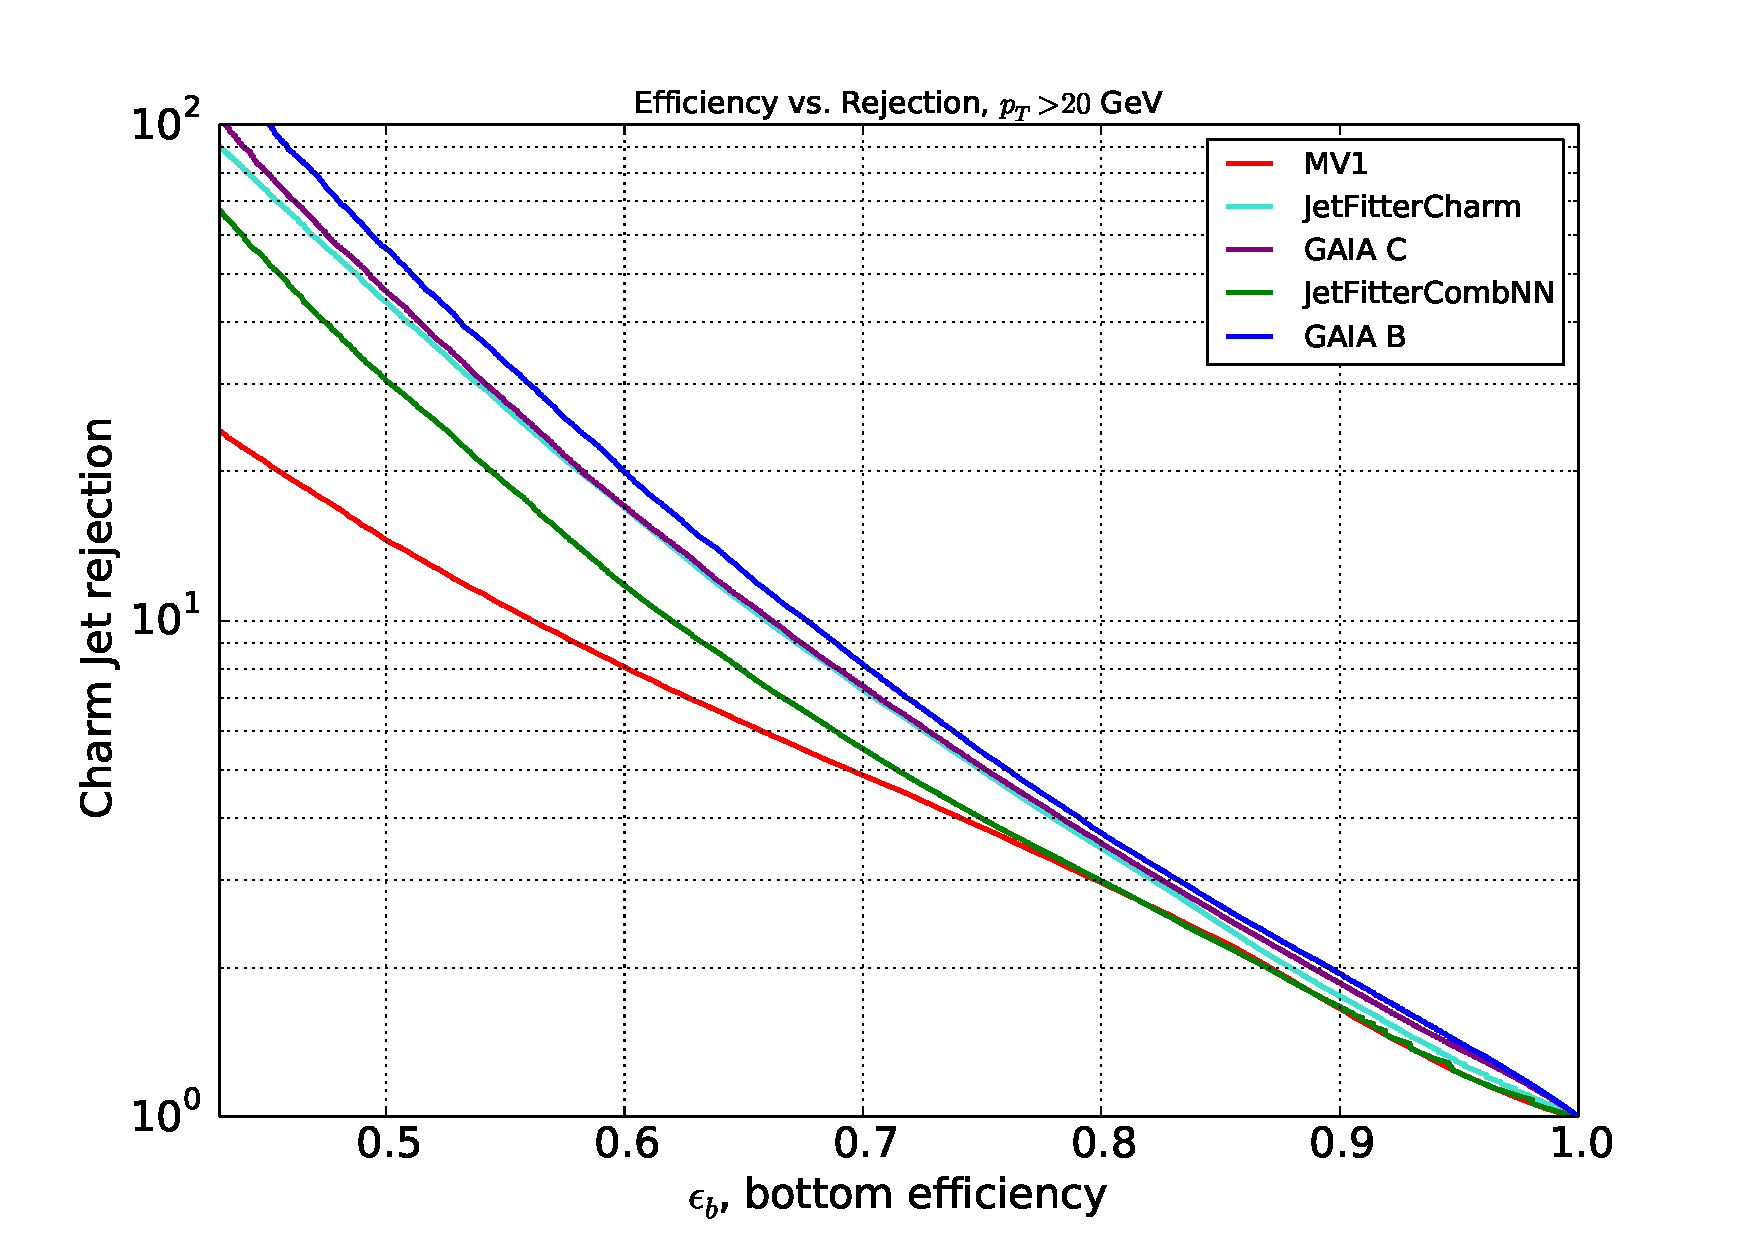
\includegraphics[width=\textwidth]{figures/btag/c_rej_ROC.pdf}
\caption[The ATLAS detector]{$c$-rejection Receiver Operating Characteristic Curve of Tagging Lineup.
\label{fig:crejROC}}
\end{figure}

\newcommand{\pt}{$p_T$ }
\subsection{Concerning \pt}


As previously stated, we concern ourselves with $p_T$ dependent performance of a tagger. That is, consider a fixed global cut on a discriminant that we have determined to yield an $\varepsilon_b$ of 0.60. If we look at specific $p_T$ ranges, how does that global performance map to the specified range? It is desirable to have a tagger exhibit flat performance across $p_T$ ranges, as this ensures that the tagger can operate in different mass and $p_T$ ranges required by different analyses. To quantify this, we take a global cut that we determine to produce a specified $\varepsilon$ over the entire sample. Then, we look at specific bins\footnote{\`{A} la a histogram} of $p_T$, and determine how that cut on discriminant performs in that particular bin. We can quantify signal efficiency in that bin, and we can also look at both types of background rejection, and see if we see a desirable relationship between $p_T$ and performance related measures. It should be noted that in all \pt dependence plots, a cut is only made on $\log(p_b/p_c)$ for simplicity.


In Figure \ref{fig:urej_fixed} we see the \pt range dependence of bottom rejection at an $\varepsilon_b =  0.70$, and 0.80 level. Clearly, GAIA B outperforms MV1 and JetFitterCombNN in each \pt bin. However, the increase in performance comes at a cost -- the \pt dependence is not flat. We can see that GAIA C shows flat performance across the \pt spectrum, sacrificing performance in lower \pt bins for flatness across the spectrum. Plots showing \pt dependence of $c$-rejection and efficiency for each operating point $\varepsilon_b = \{0.70, 0.80\}$ are included in the Appendix for the sake of brevity. 


\begin{FPfigure}
\includegraphics[width=\textwidth]{figures/btag/urej_fixedOP_70}\\
\includegraphics[width=\textwidth]{figures/btag/urej_fixedOP_80}
\caption[perf_plot]{$u$ rejection as a function of jet $p_T$, fixed efficiency cut at $\varepsilon_b = \{0.70, 0.80\}$.
\label{fig:urej_fixed}}
\end{FPfigure}

How do we get the \pt dependent dynamics we see in Figure \ref{fig:urej_fixed}? Consider the case where we fix $\varepsilon_b = 0.70$. We must examine the $\varepsilon_b$-\pt dependence in order to shed light on where this dynamic comes from.

\begin{figure}
\includegraphics[width=\textwidth]{figures/btag/beff_fixedOP_70}
\caption[perf_plot]{$b$ efficiency as a function of jet $p_T$, fixed efficiency cut at $\varepsilon = 0.70$.
\label{fig:beff_fixedOP_70}}
\end{figure}

Figure \ref{fig:beff_fixedOP_70} shows the \pt dependence of efficiency. Cross referencing between the top of Figure \ref{fig:urej_fixed} and Figure \ref{fig:beff_fixedOP_70} we can see that in each \pt bin, there seems to be a relationship between in-bin efficiency and the rejection we see, which makes sense -- rejection and efficiency are inversely correlated. 

To examine this relationship, we perform a normalization procedure as follows. First, make a fixed output cut on MV1, and examine each \pt bin to determine in-bin signal efficiency. Then for each other tagger and for each \pt bin, we determine a cut on that taggers output spectrum  that achieves the same in-bin signal efficiency as MV1. This procedure is a better indicator of how an algorithm performs, as it is less sample dependent. As we can see in Figure \ref{fig:urejmv1norm70}, 
\begin{figure}
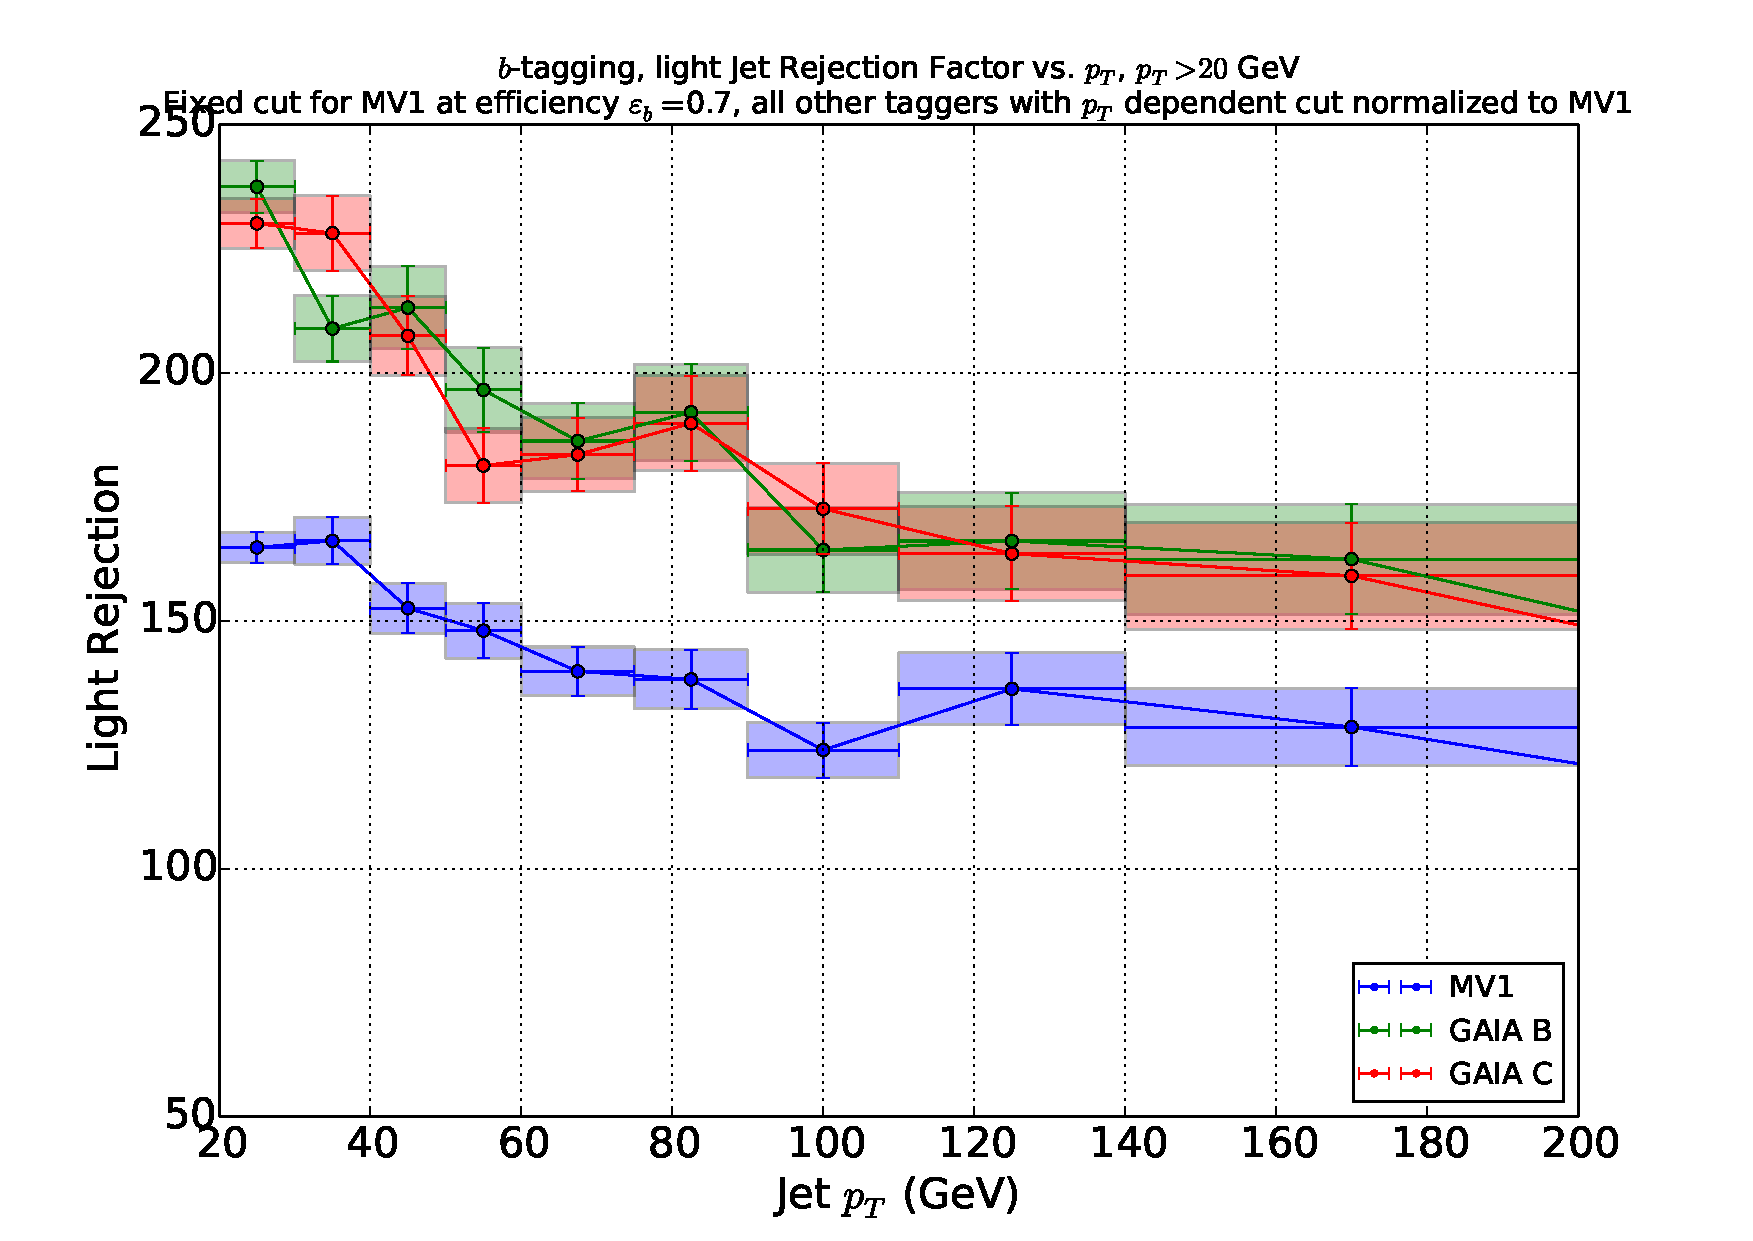
\includegraphics[width=\textwidth]{figures/btag/u_rej_mv1normalized_pTdep_70pct.pdf}
\caption[The ATLAS detector]{MV1 Normalized Performance of GAIA.
\label{fig:urejmv1norm70}}
\end{figure}
the rejection performance of GAIA B and GAIA C are nearly identical and are certainly within statistical uncertainties. Interestingly enough, both versions of GAIA are clearly above MV1 for the entire $p_T$ spectrum, indicating superior performance for every \pt range of interest. 

This indicates the possibility that different trainings of GAIA using different weighting are simply a way of implicitly making \pt dependent cuts. This warrants further investigation, as something such as a consistent way of reweighting posteriors using a $(p_T, \eta)$ polynomial would change the way reweighting is done within physics analyses.

\subsection{Using IDNE}


Using the Inverted Deep Network Encoding outlined in Chapter 3, we show performance improvements over GAIA B and GAIA C. As was evident in Figure \ref{fig:featGAIA}, GAIA with IDNE learned very informative features with respect to the structure of our dataset. This feature is not tested, and a thorough analysis of performance on a variety of problems is left as a future study. 



\begin{figure}
\includegraphics[width=\textwidth]{figures/btag/u_rej_ROC_IDNE.pdf}
\caption[The ATLAS detector]{$u$-rejection Receiver Operating Characteristic Curve of Tagging Lineup.
\label{fig:urejROCIDNE}}
\end{figure}

In Figure \ref{fig:urejROCIDNE}, we can clearly see that GAIA with IDNE is tentatively able to classify better than all other versions of GAIA, indicating a promising development.  

\begin{figure}
\includegraphics[width=\textwidth]{figures/btag/c_rej_ROC_IDNE.pdf}
\caption[The ATLAS detector]{$c$-rejection Receiver Operating Characteristic Curve of Tagging Lineup.
\label{fig:crejROCIDNE}}
\end{figure}
Figure \ref{fig:crejROCIDNE} affirms this performance increase, showing that both $u$ rejection and $c$ rejection for the $b$ tagging problem are improved when using the IDNE method of developing more informative features. 

\section{$c$-tagging}

Tagging $c$-jets is an entirely different problem than $b$-tagging. Depending on the target sample, a physicist will have to very carefully choose an operating point to maximize the rejection with respect to the sample-specific backgrounds. In particular, for a given signal efficiency, $\varepsilon_c$, a physicist will need to consider what point in rejection space is appropriate for the sample that will be used in a particular search. A natural way of condensing this information is considering signal efficiency as a surface over the space of possible background rejections for both types of background. To do this, we sample 1,000 values across the anti-$u$ discriminant and 1,000 values across the anti-$b$ discriminant, and determine the signal efficiency and both background rejections for all $1,000^2$ possible cuts on discriminant pairs. 

This process yields a densely samples surface. In order to make the surface well defined, we take a 2D cumulative maximum of $\varepsilon_c$ across rejection space starting at the highest rejection-rejection pair. If we plot this as a heat-map, we can divide two such graphics from different taggers, yielding a ratio of tagger efficiencies for each point in rejection space. 

Consider Figure \ref{fig:gbjfcphase}, which shows such a graphic for GAIA B against the current ATLAS standard for $c$-tagging, JetFitterCharm. We also see iso-$\varepsilon_c$ contours from GAIA B, showing the level curves from the original signal efficiency surface. The colors in rejection space represent the ratio of GAIA B signal efficiency to that of JetFitterCombNN. We cap the ratio at a 20\% improvement to better show regions of improvement. 

\begin{figure}[h!]
\includegraphics[width=0.9\textwidth]{figures/btagging/phase_gaia_b_versus_jfcharm.pdf}
\caption[The ATLAS detector]{Iso-$\varepsilon$ plot of GAIA B versus JetFitterCharm.
\label{fig:gbjfcphase}}
\end{figure}

In Figure \ref{fig:gcjfcphase}, we see the rejection-space $c$-tagging efficiency improvements of GAIA C with respect to JetFitterCharm. As is the case in Figure \ref{fig:gbjfcphase}, we see that the the GAIA framework provides a better signal efficiency than JetFitterCharm for every possible rejection pairing. 

\begin{figure}[h!]
\includegraphics[width=0.9\textwidth]{figures/btagging/phase_gaia_c_versus_jfcharm.pdf}
\caption[The ATLAS detector]{Iso-$\varepsilon$ plot of GAIA C versus JetFitterCharm.
\label{fig:gcjfcphase}}
\end{figure}


GAIA B was optimized for $b$ jets, and GAIA C was a more general purpose tuning. How do these tunings compare to each other? Figure \ref{fig:gbgcphase} shows us that they perform very similarly -- they are within 6\% of each other for every rejection pairing. It seems, however, that GAIA B performs very well when the desired $\varepsilon_c$ is higher, which makes sense. Since GAIA B was trained to identify $b$ jets, and since most $c$ jets are $b$-like, GAIA B is better at identifying the harder cases. Conversely, since GAIA C is more general purpose, it is better at identifying when a jet is clearly a $c$ jet. 

\begin{figure}[h!]
\includegraphics[width=0.9\textwidth]{figures/btagging/phase_gaia_b_versus_gaia_c.pdf}
\caption[The ATLAS detector]{Iso-$\varepsilon$ plot of GAIA B versus GAIA C.
\label{fig:gbgcphase}}
\end{figure}

Both tunings yield interesting results, and clearly warrant further study. In particular, we wish to consider polynomial reweightings of the posterior probability distributions according to kinematic distributions, and whether GAIA with Inverted Deep Network Encoding can offer increases in $c$-tagging performance. 





















%For each flavor $\theta$, we assume that
%\begin{equation}
%\label{eq:findingcut}
%\forall\omega\in [0,1], \exists \bar{p_\theta}\text{ such that }\int_0^{\bar{p_\theta}} f_\theta(x)dx = \omega.
%\end{equation}
%
%Since $f_\theta$ is a probability distribution, for each $\omega$ we want, the $\bar{p_\theta}$ is unique. Thus, we can define a function 







